\documentclass[conference]{IEEEtran}
\IEEEoverridecommandlockouts

\usepackage[utf8]{inputenc}
\usepackage[T1]{fontenc}
\usepackage[spanish,english]{babel}
\usepackage{cite}
\usepackage{amsmath,amssymb,amsfonts}
\usepackage{algorithmic}
\usepackage{graphicx}
\usepackage{textcomp}
\usepackage{xcolor}
\usepackage{hyperref}

\def\BibTeX{{\rm B\kern-.05em{\sc i\kern-.025em b}\kern-.08em
    T\kern-.1667em\lower.7ex\hbox{E}\kern-.125emX}}

% Terminología del pipeline (evita tipografía monoespaciada en el cuerpo)
\newcommand{\trafonormal}{tráfico normal}
\newcommand{\arpspoof}{ARP spoofing}
\newcommand{\macflood}{MAC flooding}
\newcommand{\portscan}{escaneo de puertos}
\newcommand{\arprecon}{reconocimiento ARP}
\newcommand{\victimauno}{primera víctima}
\newcommand{\victimados}{segunda víctima}

\begin{document}

\title{ARPegio: Detección No Supervisada de Anomalías L2 en LAN
IEEE~802.3 con Priorización de Alertas}

\author{
  \IEEEauthorblockN{Daniel Alonso Gracia Pinto}
  \IEEEauthorblockA{
    \textit{Redes de Computadores -- Grupo 3} \\
    \textit{Universidad Nacional de Colombia} \\
    Bogotá, Colombia \\
    dagraciap@unal.edu.co
  }
}

\maketitle
\thispagestyle{plain}
\pagestyle{plain}

% ---------------------------------------------------------------
%  ABSTRACT (English)
% ---------------------------------------------------------------
\begin{abstract}
Institutional IEEE~802.3 LANs are the operational backbone of critical
services, yet they remain largely blind to early-stage threats that
emerge below the IP layer. Attacks such as ARP spoofing, MAC flooding,
silent port scanning, and ARP reconnaissance manifest as subtle deviations
in otherwise legitimate Layer~2 traffic---deviations that
signature-based intrusion detection systems consistently fail to
capture. Existing Layer~2 security solutions either require active
agents deployed on every network node or depend on exhaustively labeled
attack datasets, rendering them impractical for real institutional
environments. This paper proposes an unsupervised anomaly detection
system anchored at the Ethernet frame level, built around a lightweight
autoencoder that learns a behavioral baseline of normal traffic without
any labeled data. A statistical threshold calibration mechanism controls
the false-positive rate without requiring attack samples, and an
automatic alert prioritization engine ranks detected anomalies by
severity, frequency, and node impact to mitigate operator alert fatigue.
A web-based operational platform (\textit{ARPegio}) integrates these
components into an analyst-facing workflow comprising monitoring,
prioritized triage, interactive laboratory replay, and an optional
AI-assisted agent in preventive and reactive modes. The system is evaluated on traffic captured in a controlled IEEE~802.3
LAN emulated with GNS3, comprising four Layer~2 attack families---ARP
spoofing, MAC flooding, port scanning, and ARP reconnaissance---and
periods of legitimate baseline traffic. From two victim-side captures,
959 temporal windows of native Ethernet features were extracted and
labeled for evaluation; model training uses normal traffic only.
Results demonstrate the viability of passive, label-free monitoring for
proactive IEEE~802.3 LAN cybersecurity, the operational usability of an
integrated analyst platform, and highlight the open research gap in
Layer~2-anchored unsupervised network intrusion detection.
\end{abstract}

\begin{IEEEkeywords}
Anomaly detection, unsupervised learning, autoencoder, IEEE~802.3,
Ethernet, ARP spoofing, NIDS, alert prioritization, decision support,
Layer~2 security.
\end{IEEEkeywords}

% ---------------------------------------------------------------
%  RESUMEN (Spanish)
% ---------------------------------------------------------------
\begin{otherlanguage}{spanish}
\renewcommand{\abstractname}{Resumen}
\begin{abstract}
Las redes LAN IEEE~802.3 institucionales constituyen el núcleo operativo
de servicios críticos, pero permanecen en gran medida ciegas ante amenazas
tempranas que se originan por debajo de la capa IP. Ataques como ARP
spoofing, MAC flooding, escaneo silencioso de puertos y reconocimiento ARP
se manifiestan como desviaciones sutiles en el tráfico legítimo de capa~2,
desviaciones que los sistemas de detección de intrusos basados en firmas
no logran capturar consistentemente. Las soluciones de seguridad existentes
para capa~2 exigen agentes activos en cada nodo o dependen de conjuntos
de datos de ataques exhaustivamente etiquetados, lo que las hace inviables
en entornos institucionales reales. Este artículo propone un sistema de
detección de anomalías no supervisado anclado en la trama Ethernet,
construido sobre un \textit{autoencoder} ligero que aprende un perfil de
normalidad del tráfico sin requerir datos etiquetados. Un mecanismo de
calibración estadística del umbral controla la tasa de falsos positivos
sin necesidad de muestras de ataque, y un motor automático de priorización
de alertas clasifica las anomalías detectadas según severidad, frecuencia
e impacto en el nodo para mitigar el \textit{alert fatigue} del operador.
Una plataforma web de operación (\textit{ARPegio}) integra estos
componentes en un flujo orientado al analista: monitoreo, \textit{triage}
priorizado, laboratorio interactivo y un agente de asistencia opcional en
modos preventivo y reactivo. El sistema se evalúa sobre tráfico capturado en una LAN IEEE~802.3
controlada emulada con GNS3, que incluye cuatro familias de ataque de
capa~2---ARP spoofing, MAC flooding, escaneo de puertos y
reconocimiento ARP---intercaladas con períodos de tráfico legítimo.
A partir de dos capturas en nodos víctima se extrajeron 959 ventanas
temporales de \textit{features} Ethernet nativas, etiquetadas
únicamente para evaluación; el entrenamiento emplea solo tráfico normal.
Los resultados demuestran la viabilidad del monitoreo pasivo sin etiquetas
para la ciberseguridad proactiva de redes LAN IEEE~802.3, la utilidad
operativa de una plataforma integrada para el analista, e identifican
la brecha de investigación abierta en detección no supervisada anclada
en capa~2 Ethernet.
\end{abstract}

\renewcommand{\IEEEkeywordsname}{Palabras clave}
\begin{IEEEkeywords}
Detección de anomalías, aprendizaje no supervisado, \textit{autoencoder},
IEEE~802.3, Ethernet, ARP spoofing, NIDS, priorización de alertas,
soporte a la decisión, seguridad en capa~2.
\end{IEEEkeywords}
\end{otherlanguage}

% ---------------------------------------------------------------
%  I. INTRODUCCIÓN
% ---------------------------------------------------------------
\section{Introducción}

Las redes LAN IEEE~802.3 institucionales constituyen el núcleo operativo
de servicios críticos, exigiendo niveles óptimos de seguridad y
disponibilidad continua. Sin embargo, los ataques tempranos, tales como el escaneo silencioso de
puertos, el reconocimiento ARP, el ARP spoofing y el MAC flooding, se
camuflan hábilmente como variaciones sutiles del tráfico legítimo. Estas amenazas logran establecerse en la red antes de que el
sistema advierta que está bajo ataque~\cite{tufan2021}. Ante este
panorama adverso, los sistemas de detección de intrusos basados en
firmas fallan consistentemente frente a vulnerabilidades desconocidas o
amenazas adaptativas, evidenciando la necesidad de transitar hacia
enfoques centrados en el comportamiento de la red~\cite{gamage2020}.

A pesar de la urgencia de este problema, persisten dos brechas concretas
en la literatura actual. La primera radica en que los estándares de
\textit{feature selection} para plataformas NIDS se encuentran
fuertemente anclados en flujos IP, empleando protocolos como NetFlow en
las capas~3 y~4. Esta perspectiva ignora sistemáticamente la capa~2
Ethernet, siendo este el nivel exacto de la arquitectura donde ocurren
ataques de suplantación como el ARP spoofing y la saturación de tablas
mediante MAC flooding; además, las características basadas en flujos
presentan un retraso inherente frente a la captura directa a nivel de
paquete~\cite{sarhan2022,he2023}. La segunda brecha evidencia que las
soluciones de seguridad existentes diseñadas para la capa~2 requieren
agentes activos instalados en cada nodo o dependen de vastos conjuntos
de datos exhaustivamente etiquetados, exigencias técnicas que las hacen
completamente inviables para su despliegue en entornos institucionales
reales~\cite{morsy2022,sakhawat2019}.

Por consiguiente, no existe en la actualidad una solución que combine
simultáneamente cuatro factores fundamentales: una detección no supervisada
anclada en la capa~2 IEEE~802.3; un monitoreo verdaderamente pasivo y
sin agentes que entrene su modelo utilizando únicamente el tráfico normal
de la red; un motor automático que clasifique las amenazas para reducir
el \textit{alert fatigue} que abruma a los operadores de
seguridad~\cite{tariq2025}; y una capa de presentación que traduzca esos
resultados en un flujo operativo accionable para el analista, más allá de
métricas aisladas o informes estáticos. Frente a esta carencia, este
proyecto propone un \textit{autoencoder} no supervisado diseñado para
aprender un perfil robusto de normalidad del tráfico Ethernet y detectar
desviaciones significativas, complementado con un motor de priorización
basado en la severidad, frecuencia e impacto de las anomalías, y con la
plataforma \textit{ARPegio} como interfaz de operación y validación. La
elección de un método no supervisado se justifica en la realidad operativa: en una LAN
institucional, etiquetar todas las variaciones de tráfico malicioso es
una tarea inviable. Si bien la literatura reconoce que los métodos
supervisados suelen igualar o superar el rendimiento de los no
supervisados en entornos de prueba estructurados, el enfoque no
supervisado no se plantea aquí como superior en abstracto, sino como la
única alternativa técnica viable frente a la ausencia absoluta de
etiquetas en este escenario real~\cite{gamage2020}.

En respuesta a estas limitaciones, el presente artículo introduce cuatro
contribuciones específicas. Primero, se plantea una arquitectura de
monitoreo pasivo que captura tramas Ethernet en un punto de visibilidad
del segmento LAN---análogo a un puerto espejo (\textit{SPAN})---sin
requerir agentes en los nodos víctima. Segundo, se desarrolla un modelo de
detección de anomalías no supervisado fundamentado en un \textit{autoencoder},
el cual emplea una calibración de umbral estadística sin depender de datos
etiquetados. Tercero, se integra un motor de priorización automático de
alertas configurado según la severidad, frecuencia y el nivel de impacto
en el nodo afectado. Cuarto, se diseña e implementa la plataforma web
\textit{ARPegio}, que articula monitoreo, \textit{triage} priorizado,
laboratorio interactivo con inferencia en el cliente y asistencia del
operador mediante un agente conversacional en modos preventivo y
reactivo, cerrando el ciclo entre la evaluación experimental y la decisión
en el SOC. El diseño propuesto se fundamenta en criterios
estrictos que guían toda la metodología: la resiliencia ante la
manipulación adversaria para evitar la evasión del
modelo~\cite{he2023}, la viabilidad computacional para operar ágilmente
en entornos reales~\cite{injadat2021}, y la reproducibilidad basada en
el rigor experimental~\cite{yang2022}. El resto del artículo se organiza
de la siguiente manera: la Sección~II revisa los trabajos relacionados;
la Sección~III describe la metodología propuesta; la Sección~IV detalla
la configuración experimental; la Sección~V presenta el diseño de la
plataforma web de operación; la Sección~VI expone y discute los
resultados; y la Sección~VII concluye el trabajo.

% ---------------------------------------------------------------
%  II. TRABAJOS RELACIONADOS
% ---------------------------------------------------------------
\section{Trabajos Relacionados}
 
\subsection{NIDS no supervisado}
El enfoque no supervisado para sistemas de detección de intrusos en redes
(NIDS) ha ganado una tracción significativa, pero presenta limitaciones
persistentes en términos de generalización y viabilidad según el contexto
de despliegue. Como punto de partida en este debate, Gamage y Samarabandu
establecen que los métodos no supervisados son viables en la práctica,
aunque suelen tener un rendimiento inferior en los \textit{benchmarks}
tradicionales frente a los modelos supervisados; no obstante, su
verdadera ventaja competitiva radica en contextos operativos que carecen
de etiquetas~\cite{gamage2020}. Posteriormente, Griffin et al. presentan
un \textit{ensemble} de \textit{autoencoders} para operar en tiempo real
sobre arquitecturas SDN~\cite{griffinyang2022}. Aunque efectivo, este
modelo presenta una complejidad computacional mayor que la nuestra y
asume una infraestructura SDN que rara vez está disponible en una LAN
institucional típica. Por su parte, Antunes et al. realizan un riguroso
\textit{benchmark} de métodos de \textit{deep learning} para NIDS,
evidenciando claras inconsistencias y un bajo rendimiento al momento de
detectar ataques de infiltración~\cite{antunes2022}. Esto subraya la
necesidad de un anclaje más profundo en la red. La limitación común de
estos trabajos es que operan exclusivamente sobre flujos IP (como
NetFlow), ignorando el nivel base donde los ataques internos realmente
se originan.
 
\subsection{LAN institucional}
La literatura que aborda entornos de redes institucionales reales es
escasa y habitualmente presenta restricciones críticas relacionadas con
la escala de la red o la dependencia absoluta de la supervisión de datos.
Tufan et al. validan la existencia de esta problemática en entornos de
producción mediante pruebas con ataques de reconocimiento en una red
institucional real, confirmando la vulnerabilidad del entorno, aunque
basan su propuesta en enfoques supervisados que limitan su aplicabilidad
autónoma~\cite{tufan2021}. En un esfuerzo por abordar despliegues de
mayor tamaño, Sun et al. proponen el uso de \textit{Segmented Federated
Learning} para LANs a gran escala~\cite{sun2021ojcoms}. Si bien este
enfoque escala adecuadamente, exige una coordinación estricta entre
nodos, lo cual resulta inviable sin una infraestructura federada
dedicada. Dentro de estas redes institucionales, el vector de ataque más
crítico e ignorado ocurre de manera insidiosa en la capa~2 Ethernet.
 
\subsection{Detección en capa 2 IEEE 802.3}
La investigación enfocada en la capa~2 existe, pero la mayoría de las
soluciones dependen de la modificación de protocolos, agentes activos o
esquemas estrictamente supervisados. Morsy y Nashat proponen D-ARP para
mitigar el \textit{ARP spoofing}, siendo esta una solución activa que
altera el comportamiento estándar del protocolo y exige un control total
sobre la infraestructura subyacente~\cite{morsy2022}. Prasad y Chandra
combinan técnicas de aprendizaje automático con \textit{device profiling}
para lograr un objetivo similar~\cite{prasad2022}; sin embargo, su
enfoque es supervisado y demanda la instalación de aplicaciones cliente
o agentes por nodo. El modelo más cercano a nuestra propuesta es el de
Sun et al., quienes utilizan un \textit{autoencoder} para procesar
actividad ARP sospechosa~\cite{sun2022ccnc}. Aunque meritorio, dicho
trabajo carece de un anclaje explícito al estándar IEEE~802.3 y no
incluye un motor de priorización. Finalmente, Sakhawat et al. definen
características ARP en una LAN conmutada mediante una solución basada en
agentes~\cite{sakhawat2019}, un obstáculo de implementación que nuestra
propuesta supera al basarse netamente en monitoreo pasivo. Ninguno de
estos trabajos aborda el problema de la sobrecarga operativa generada por
las alertas, el eslabón final que completa la brecha hacia una solución
autónoma.
 
\subsection{Priorización de alertas en SOCs}
La priorización de alertas se reconoce ampliamente como un desafío
crítico, pero las alternativas existentes en la literatura dependen
excesivamente de la intervención humana o conjuntos de datos previamente
etiquetados, factores incompatibles con un \textit{pipeline} analítico
totalmente automático. Tariq et al. definen la \textit{alert fatigue}
como un cuello de botella paralizante en los SOCs y determinan que la
severidad, frecuencia e impacto son los criterios definitivos para
abordarla~\cite{tariq2025}, premisa que motiva directamente el diseño de
nuestro motor de priorización. En paralelo, Aminanto et al. utilizan un
\textit{autoencoder} apilado para reducir los falsos positivos antes de
la fase de priorización~\cite{aminanto2020}; esto representa una
arquitectura combinada alternativa a nuestra propuesta, pero delega el
\textit{autoencoder} a un mero rol de filtro y no como el motor de
detección principal. De manera similar, Jalalvand et al. estructuran un
marco integral de criterios para la priorización en
SOCs~\cite{jalalvand2024}, que si bien fundamenta los parámetros que
adopta nuestro motor, está fuertemente orientado a facilitar la toma de
decisiones humana en esquemas colaborativos. Por último, Carrera et al.
implementan detección \textit{near real-time} combinando múltiples
algoritmos no supervisados~\cite{carrera2022}, resultando en una
arquitectura sustancialmente más compleja que nuestra propuesta, y que
descartamos para nuestro contexto debido al alto \textit{overhead}
computacional que introduce en la red.
 
La literatura existente logra colectivamente avances significativos en
modelos de \textit{deep learning}, visibilidad de capa de enlace y la
gestión de la fatiga de alertas, pero invariablemente aborda estos retos
de forma aislada o asumiendo infraestructuras fuertemente supervisadas o
intervenidas. La brecha específica que ningún trabajo previo llena, y que
esta investigación resuelve integralmente, es la consolidación de un
sistema NIDS para redes IEEE~802.3 que opere de forma puramente no
supervisada, sin requerir agentes en los nodos, que integre de forma
nativa un motor de priorización automático para garantizar la viabilidad
operativa en entornos reales, y que disponga de una plataforma de
operación que haga interpretables y accionables sus resultados para el
analista de seguridad.

% ---------------------------------------------------------------
%  III. METODOLOGÍA
% ---------------------------------------------------------------
\section{Metodología}

\subsection{Visión general del sistema}
El diseño metodológico propuesto se estructura como un \textit{pipeline}
de extremo a extremo compuesto por cuatro etapas estrictamente
secuenciales. La primera etapa realiza la captura pasiva del tráfico
Ethernet en el segmento protegido, emulando el despliegue de un IDS
pasivo con visibilidad de capa~2. La segunda fase ejecuta la extracción
y normalización de características nativas de tramas IEEE~802.3.
Posteriormente, la tercera etapa detecta las desviaciones mediante un
modelo \textit{autoencoder} de aprendizaje no supervisado. Finalmente,
la cuarta fase procesa estos eventos a través de un motor de
priorización automática de alertas, evaluadas según su severidad,
frecuencia e impacto en el nodo. Una quinta capa de operación---la
plataforma \textit{ARPegio} descrita en la Sección~V---expone los
resultados del \textit{pipeline} al analista sin alterar el entrenamiento
ni la inferencia del modelo. Durante el entrenamiento y la
calibración del umbral, ninguna etapa consume etiquetas de ataque; las
etiquetas temporales del \textit{dataset} experimental se reservan
exclusivamente para la evaluación posterior del rendimiento.

\subsection{Arquitectura del autoencoder}
La detección de desviaciones conductuales se fundamenta en una
arquitectura \textit{encoder-decoder} simétrica y no supervisada. El
componente \textit{encoder} recibe el vector de características
normalizado y, mediante dos capas densas con funciones de activación
ReLU, realiza una reducción dimensional progresiva hacia un espacio
latente, específicamente con proyecciones $11 \to 8 \to 4$ en el
\textit{encoder} y simétricas $4 \to 8 \to 11$ en el \textit{decoder};
dicho espacio condensa la representación comprimida y fundamental del
comportamiento normal de la red LAN. En contraposición, el bloque
\textit{decoder} procesa este espacio latente para reconstruir de forma
simétrica el vector original en la salida. El modelo se optimiza
empleando el error cuadrático medio (\textit{Mean Squared Error}, MSE)
como función de pérdida, entrenándose exclusivamente con tráfico
legítimo. Debido a que la red aprende únicamente las regularidades
estadísticas de la normalidad, la presencia de tráfico anómalo se
manifiesta a través de un error de reconstrucción elevado. Este enfoque
basado en un \textit{autoencoder} monolítico se elige por su simplicidad
analítica y efectividad para establecer líneas base de seguridad sin
requerir etiquetas~\cite{li2020}, consolidando al MSE como una métrica
robusta e interpretable para la cuantificación de anomalías en entornos
de red~\cite{song2021}. Asimismo, frente a soluciones complejas basadas
en un \textit{ensemble} de múltiples \textit{autoencoders} orientados a
redes lógicas~\cite{griffinyang2022}, la arquitectura propuesta minimiza
el \textit{overhead} computacional y resulta óptima y suficiente para
representar las dinámicas de la capa de enlace sin comprometer los
recursos del sistema.

La adopción de esta arquitectura modular obedece directamente a la
necesidad de establecer un marco de trabajo estructurado que garantice un
estricto rigor experimental y metodológico en la evaluación de sistemas
de detección~\cite{yang2022}. Asimismo, la estructuración en un
\textit{pipeline} multi-etapa resulta esencial para asegurar la
viabilidad computacional del modelo, dado que permite reducir la
complejidad general del procesamiento continuo y viabiliza su despliegue
ágil en entornos de red reales~\cite{injadat2021}.

\subsection{Adquisición de datos en laboratorio virtual}
Para materializar el monitoreo pasivo de capa~2 sin agentes en las
víctimas, se emuló un segmento LAN IEEE~802.3 en GNS3 sobre Fedora,
interconectando dos nodos Alpine Linux (víctimas), un nodo Kali Linux
(atacante) y un \textit{Open vSwitch} (OVS) como conmutador central del
segmento 192.168.1.0/24. Las direcciones estáticas asignadas
fueron 192.168.1.10 (Alpine-1), 192.168.1.20
(Alpine-2) y 192.168.1.99 (Kali). La conectividad ICMP entre
víctimas se verificó antes de iniciar la recolección.

La captura no se realizó en el nodo atacante---escenario poco realista
para un IDS de producción---sino en los enlaces físicos simulados entre
cada víctima y el OVS, mediante la captura integrada de GNS3 a nivel de
hipervisor. Este procedimiento replica un punto de observación neutral
del segmento, equivalente operativamente a un puerto espejo (\textit{SPAN})
o a un TAP de red: el sensor observa el tráfico que llega a cada
estación protegida, incluyendo tramas ARP, \textit{broadcasts} y tráfico
inter-víctima que un host individual no necesariamente genera. Se
descartó depender de \textit{tcpdump} dentro de Alpine---sin paquetes
disponibles offline---y de configuraciones de \textit{port mirroring}
manuales sobre el OVS embebido de GNS3, que resultaron frágiles frente a
capturas promiscuas desde Kali.

La sesión experimental se ejecutó como una única captura continua por
víctima, con fases alternadas de tráfico legítimo y ataques controlados
desde Kali. La Tabla~\ref{tab:secuencia_ataques} resume la secuencia.
Entre fases se insertaron períodos de tráfico normal (ICMP entre
víctimas) para delimitar temporalmente cada familia de ataque en las
capturas, de modo que el \textit{dataset} refleje la
mezcla realista entre baseline y anomalías observada en operación.

\begin{table}[htbp]
\caption{Secuencia experimental de recolección en GNS3}
\label{tab:secuencia_ataques}
\centering
\renewcommand{\arraystretch}{1.15}
\begin{tabular}{clll}
\hline
\textbf{Fase} & \textbf{Duración} & \textbf{Actividad} & \textbf{Herramienta} \\
\hline
1 & $\sim$3 min & Tráfico normal (ICMP) & \textit{ping} en Alpine \\
2 & $\sim$2 min & ARP spoofing / MITM & \textit{arpspoof} en Kali \\
3 & $\sim$1 min & Pausa normal & \textit{ping} en Alpine \\
4 & $\sim$1 min & MAC flooding & \textit{macof} en Kali \\
5 & $\sim$1 min & Pausa normal & \textit{ping} en Alpine \\
6 & $\sim$3--5 min & Port scan & \textit{nmap} en Kali \\
7 & --- & ARP reconnaissance & \textit{arping} en Kali \\
\hline
\end{tabular}
\end{table}

Las capturas resultantes en ambos nodos víctima
contienen $\approx$24\,000 tramas Ethernet cada una, con una duración
total de 34.6~minutos y \textit{link-type} EN10MB, confirmando análisis a
nivel de trama IEEE~802.3.

\subsection{Selección de características y preprocesamiento}
El vector de \textit{features} se limita a métricas nativas de capa~2
extraídas con Scapy sobre ventanas temporales de 50 tramas consecutivas.
Las dimensiones implementadas son: (i)~tasa de tramas ARP;
(ii)~ratio \textit{ARP request/reply}; (iii)~entropía de direcciones MAC
origen; (iv)~conteo de MAC origen y destino
únicas; (v)~estadísticos de longitud de trama Ethernet
(media, desviación estándar, mínimo y máximo); y (vi)~ratio de
tramas broadcast. Esta selección cubre directamente las familias de
ataque evaluadas: el ARP spoofing eleva la tasa ARP con bajo
\textit{request/reply}; el MAC flooding concentra la entropía MAC
y el número de direcciones origen únicas; el escaneo de puertos reduce
la variabilidad de longitud de trama; y el reconocimiento ARP mantiene
tasa ARP elevada con patrón distinto al envenenamiento activo.
Este anclaje en la capa de enlace cubre el punto ciego metodológico
identificado en sistemas basados exclusivamente en flujos
IP~\cite{sarhan2022,sun2022ccnc}.

Respecto al preprocesamiento, se aplica una normalización \textit{min-max}
para escalar los datos al rango $[0,1]$. Las ventanas se etiquetan
post-\textit{hoc} según el timestamp central de cada ventana y los
intervalos temporales de la Tabla~\ref{tab:secuencia_ataques}, con cinco
clases: \trafonormal, \arpspoof, \macflood,
\portscan{} y \arprecon. El entrenamiento del
\textit{autoencoder} y la calibración de $\theta$ emplean únicamente
ventanas de \trafonormal; las etiquetas de ataque se reservan para medir
\textit{recall} y \textit{precision} en evaluación. Por política de
diseño, no se realiza imputación de valores faltantes; las tramas sin
capa Ethernet se descartan al particionar ventanas.

\subsection{Calibración estadística del umbral}
El mecanismo de calibración del sistema para la identificación de
desviaciones se estructura en tres pasos analíticos. Primero, una vez
finalizado el entrenamiento del \textit{autoencoder}, se calcula el
error de reconstrucción sobre un conjunto de validación compuesto
íntegramente por tráfico normal que el modelo no ha visto previamente.
Este procedimiento permite extraer la distribución empírica del error
inherente al comportamiento legítimo de la red. Segundo, el umbral de
decisión $\theta$ se fija dinámicamente seleccionando un percentil
superior de esta distribución empírica, típicamente el percentil~95
o~99. Durante la fase de inferencia, cualquier muestra cuyo error de
reconstrucción supere estrictamente a $\theta$ se clasifica de forma
automática como una anomalía. Este enfoque garantiza la detección sin
requerir una sola muestra de ataque en la fase de
ajuste~\cite{zavrak2020}. Tercero, la adopción de este límite cuenta con
una profunda justificación estadística, dado que el percentil elegido
permite controlar de manera matemática y directa la tasa de falsos
positivos proyectada sobre el tráfico normal de la LAN~\cite{zhang2023}.
La elección de esta calibración estadística por percentil, en claro
contraste con alternativas que emplean umbrales numéricos fijos o
algoritmos de \textit{clustering} en el espacio latente, se fundamenta
en su alta interpretabilidad probabilística y su nula dependencia de
datos etiquetados~\cite{maleki2021}. El valor paramétrico exacto del
percentil utilizado constituye un hiperparámetro que se detalla en la
configuración experimental.

\subsection{Motor de priorización de alertas}
El motor de priorización evalúa cada alerta generada asignándole un
puntaje compuesto derivado de tres dimensiones independientes. La
primera dimensión es la severidad, definida como la magnitud del error
de reconstrucción que supera el umbral estadístico $\theta$, normalizada
al rango $[0,1]$. La segunda dimensión corresponde a la frecuencia, la
cual cuantifica el número de alertas emitidas por un mismo nodo origen
dentro de una ventana temporal deslizante. La tercera dimensión evalúa
el impacto, clasificando el nodo afectado según su rol jerárquico dentro
de la topología de la red, otorgando mayor peso a servidores críticos,
seguidos de estaciones cliente y dispositivos IoT. El puntaje de prioridad final se calcula como una suma ponderada de estas tres
métricas, con pesos configurables directamente por el operador de
seguridad. En la implementación de referencia se fijaron
$w_s=0{,}5$, $w_f=0{,}3$ y $w_i=0{,}2$, con
\begin{equation}
\label{eq:priority}
P = w_s \cdot s + w_f \cdot f + w_i \cdot i,
\end{equation}
donde $s=\min(e/\theta,\,1)$ es la severidad (error de reconstrucción $e$
respecto al umbral $\theta$), $f$ es la fracción de ventanas anómalas en
una ventana deslizante de $W{=}10$ por fuente de captura, e $i$ es el
impacto operacional. Dado que los nodos del laboratorio son clientes
homogéneos (Alpine Linux), el impacto se aproxima mediante pesos fijos
por familia de amenaza inferida a partir de \textit{features} L2
(\macflood: 1.0; \arpspoof: 0.9; \portscan: 0.7;
\arprecon: 0.6; desconocido: 0.5), sin emplear etiquetas
en tiempo de inferencia. La familia de amenaza se infiere mediante reglas
umbral fijas evaluadas en cascada sobre las mismas \textit{features} L2:
(i)~si el conteo de MAC origen únicas $\geq 20$, se clasifica como
\macflood; (ii)~si no, y la tasa ARP $\geq 0{,}5$, entonces
ratio petición-respuesta ARP $< 1$ indica \arpspoof{} y, en caso
contrario, \arprecon; (iii)~si no, y la desviación estándar de longitud
de trama $< 5$, se asigna \portscan; (iv)~en cualquier otro caso, la alerta queda
como \textit{desconocida}. No se emplea aprendizaje supervisado ni
\textit{clustering} en esta etapa: son heurísticas deterministas alineadas
con las señales dominantes de cada familia descritas en la subsección de
selección de características y preprocesamiento.

El diseño de este mecanismo se fundamenta en las necesidades operativas
de los Centros de Operaciones de Seguridad (SOCs), adoptando los
criterios definitivos establecidos en la literatura especializada para
mitigar la fatiga de alertas~\cite{tariq2025,jalalvand2024}. A
diferencia de enfoques alternativos que emplean \textit{autoencoders}
como filtros previos para reducir falsos positivos antes de la
priorización~\cite{aminanto2020}, o de arquitecturas
\textit{near real-time} que introducen un alto \textit{overhead}
computacional en la red~\cite{carrera2022}, el motor propuesto procesa
el flujo de manera automatizada sin requerir etiquetas ni intervención
humana. Finalmente, la implementación de la ventana temporal deslizante
permite correlacionar eventos continuos, facilitando la detección de
patrones de ataque sostenidos y adaptativos que, de otro modo, se
registrarían como alertas individuales inofensivas de muy baja
severidad.

% ---------------------------------------------------------------
%  IV. CONFIGURACIÓN EXPERIMENTAL
% ---------------------------------------------------------------
\section{Configuración Experimental}

\subsection{Dataset L2 generado}
A partir de las dos capturas en nodos víctima se derivó un conjunto de
959 ventanas etiquetadas mediante el \textit{pipeline} descrito en la
Sección~III. Cada fila corresponde a
una ventana de 50 tramas consecutivas y a las 11 \textit{features}
numéricas de capa~2, más marcas temporales de inicio y fin, identificador
de la fuente de captura y etiqueta de evaluación. La Tabla~\ref{tab:distribucion_labels} resume la
distribución resultante tras combinar ambas perspectivas de captura.

\begin{table}[htbp]
\caption{Distribución de ventanas etiquetadas (959 en total)}
\label{tab:distribucion_labels}
\centering
\renewcommand{\arraystretch}{1.15}
\begin{tabular}{lrr}
\hline
\textbf{Clase de tráfico} & \textbf{Ventanas} & \textbf{Señal L2 dominante} \\
\hline
Tráfico normal      & 116 & Baseline ICMP / tráfico legítimo \\
ARP spoofing  &   6 & Alta tasa ARP, bajo ratio req./reply \\
MAC flooding  & 795 & 50 MACs únicas, entropía MAC $\approx 3.91$ \\
Escaneo de puertos  &  36 & Baja variabilidad de longitud de trama \\
Reconocimiento ARP  &   6 & Tasa ARP $=1.0$, patrón de sondeo \\
\hline
\end{tabular}
\end{table}

El desbalance hacia \macflood{} refleja la naturaleza de ráfaga
del ataque \textit{macof}: $\approx$2.5~s de inundación generaron cientos
de ventanas consecutivas con 50 direcciones MAC distintas por ventana.
Las clases ARP (\arpspoof{} y \arprecon) concentran
pocas ventanas pero exhiben separación clara en tasa ARP frente
a \trafonormal. La perspectiva de la \victimados{} aportó 75 ventanas
de \trafonormal{} adicionales frente a 41 de la \victimauno, lo que
refuerza la línea base de entrenamiento no supervisado.

\subsection{Protocolo de entrenamiento y evaluación}
El protocolo experimental distingue explícitamente entre uso de etiquetas
en entrenamiento y en evaluación:
\begin{itemize}
\item \textbf{Entrenamiento:} solo ventanas de \trafonormal.
\item \textbf{Validación (umbral $\theta$):} subconjunto de ventanas de
\trafonormal{} no vistas en entrenamiento (percentil~95 del error MSE).
\item \textbf{Evaluación:} conjunto completo con las cinco clases, para
medir detección de anomalías por familia de ataque.
\end{itemize}
Las etiquetas temporales se derivaron del instante central de cada
ventana y de los intervalos de la sesión GNS3; no intervienen en el
ajuste del \textit{autoencoder}. El entorno de implementación emplea
Python~3.12, Scapy, pandas, scikit-learn (\textit{MinMaxScaler}),
PyTorch y \textit{uv} para reproducibilidad. El entrenamiento utiliza
33 ventanas de \trafonormal{} de la \victimauno; ocho ventanas normales
restantes de la misma fuente calibran $\theta$ (percentil~95). La
evaluación se realiza sobre 144 ventanas de la \victimados{} no vistas
en entrenamiento, con submuestreo de \macflood{} a 116 ventanas
para equilibrar la comparación por clase, igualando así el número de
ventanas de la clase dominante al total de ventanas de \trafonormal{}
disponibles (116). El optimizador empleado es Adam
con tasa de aprendizaje $lr = 1 \times 10^{-3}$, tamaño de lote de 16
ventanas y 100 épocas de entrenamiento. La ventana deslizante del motor
de priorización se fijó en $W = 10$. La implementación se organiza en
tres componentes funcionales: entrenamiento del \textit{autoencoder},
motor de priorización heurística y emisión de alertas ordenadas. Para exponer
estos resultados a un operador de seguridad sin depender del entorno de
entrenamiento, se desarrolló además la plataforma web
\textit{ARPegio}, descrita en la Sección~V.

% ---------------------------------------------------------------
%  V. DISEÑO DE LA PLATAFORMA
% ---------------------------------------------------------------
\section{Diseño de la Plataforma}

Para trasladar el \textit{pipeline} de detección L2 a un entorno
operativo comprensible por analistas, se implementó \textit{ARPegio}, una
aplicación web estática que incorpora las métricas de evaluación, la cola
de alertas priorizadas, los puntajes por ventana y los escenarios de
laboratorio producidos por el entrenamiento y la priorización. La
interfaz no reimplementa el entrenamiento ni la extracción de
\textit{features}: actúa como capa de visualización, \textit{triage} y
experimentación que cierra el ciclo entre la evaluación offline y la
toma de decisiones del SOC. La demo pública se despliega en la Web
\footnote{\url{https://vethariel.github.io/ARPegio/}}, lo que
permite reproducir la experiencia sin instalar componentes de inferencia
en el servidor.

\subsection{Arquitectura de la interfaz}
La plataforma se organiza en seis vistas navegables desde una barra
lateral persistente: \textbf{Monitor}, \textbf{Red}, \textbf{Alertas},
\textbf{Laboratorio}, \textbf{Agente} y \textbf{Ajustes}. Al iniciar,
la aplicación carga los resultados del \textit{pipeline} y deriva
métricas agregadas---AUC-ROC, umbral $\theta$, matriz de confusión por
percentil y resúmenes de alertas---que alimentan la interfaz dinámica.
Esta separación entre el procesamiento experimental del modelo y la capa
de presentación mantiene el rigor del entrenamiento mientras ofrece
interactividad al operador. La Fig.~\ref{fig:platform_monitor} ilustra la
vista \textbf{Monitor}, punto de entrada del tablero operativo.

\begin{figure}[htbp]
\centering
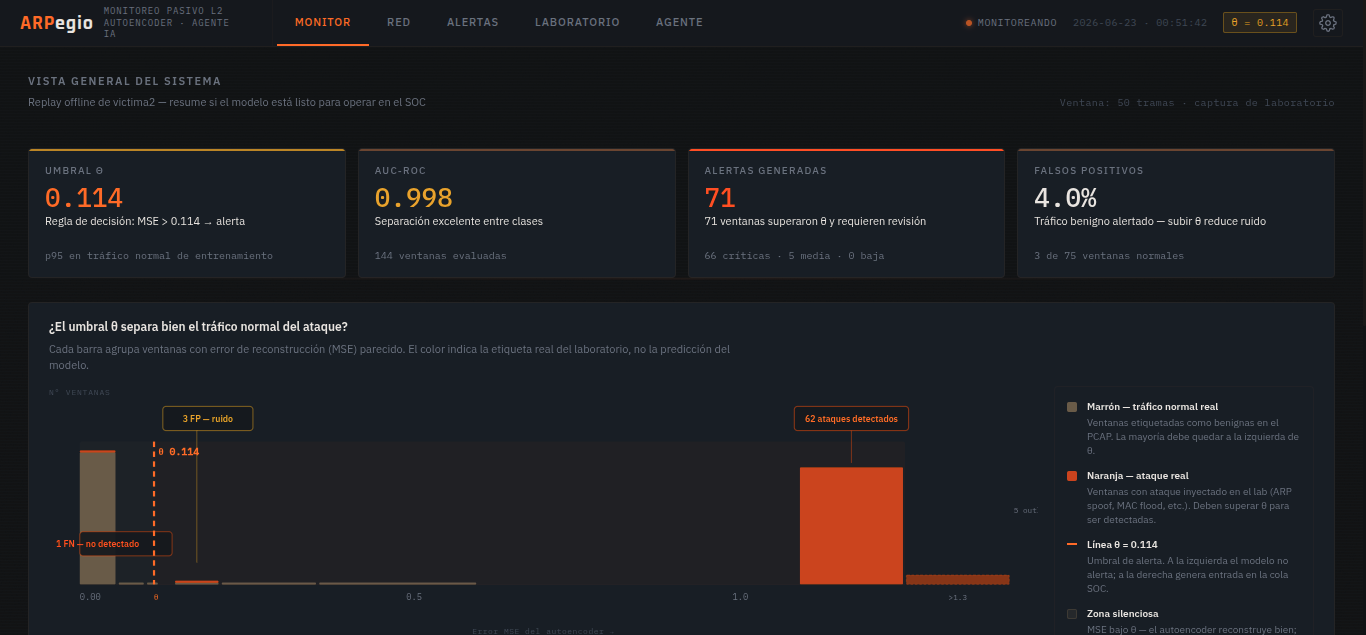
\includegraphics[width=\linewidth]{figs/vistamonitor.png}
\caption{Vista Monitor: indicadores del \textit{pipeline}, distribución
del error de reconstrucción y exploración de percentiles de $\theta$.}
\label{fig:platform_monitor}
\end{figure}

\subsection{Monitoreo, red y cola de alertas}
La vista \textbf{Monitor} resume el estado del modelo tras el
\textit{replay} offline de la \victimados: AUC-ROC, número de alertas,
tasa de falsos positivos y un histograma que contrasta el error MSE
con la etiqueta real de laboratorio (no con la predicción del modelo).
Un control deslizante permite simular distintos percentiles de $\theta$
y observar el trade-off TN/FP/FN/TP sin reentrenar.

La vista \textbf{Red} representa la topología GNS3 del segmento
192.168.1.0/24---nodos víctima Alpine, nodo atacante Kali y
conmutador OVS---junto con una línea temporal de ventanas etiquetadas
de la sesión experimental. La Fig.~\ref{fig:platform_network}
corresponde a este módulo de contexto espacio-temporal.

La vista \textbf{Alertas} materializa la salida del motor de
priorización: tabla ordenada por puntaje $P$, filtros por severidad y
familia de ataque, y panel de detalle con el vector de \textit{features}
L2 de la ventana seleccionada. Las tres alertas de mayor prioridad se
destacan también en \textbf{Monitor} como punto de entrada al
\textit{triage}. La Fig.~\ref{fig:platform_alerts} muestra la cola
priorizada y el detalle de una ventana.

\begin{figure}[htbp]
\centering
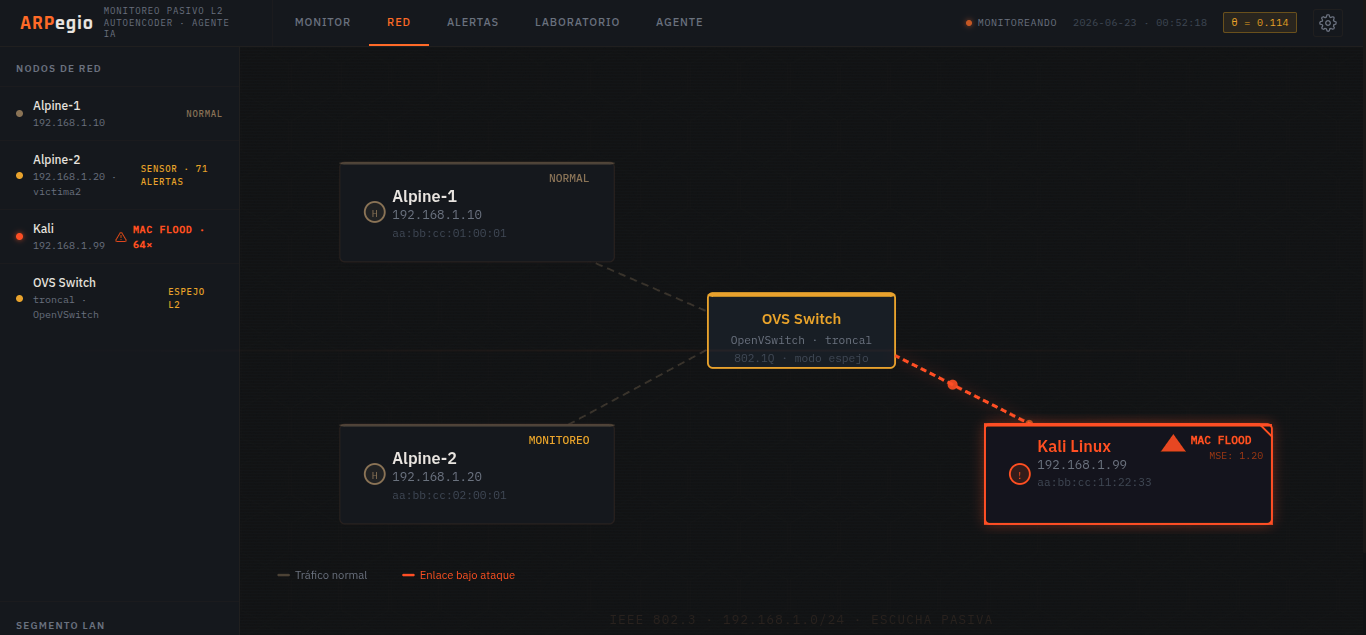
\includegraphics[width=\linewidth]{figs/topologiared.png}
\caption{Vista Red: topología del laboratorio y secuencia temporal de
ventanas etiquetadas.}
\label{fig:platform_network}
\end{figure}

\begin{figure}[htbp]
\centering
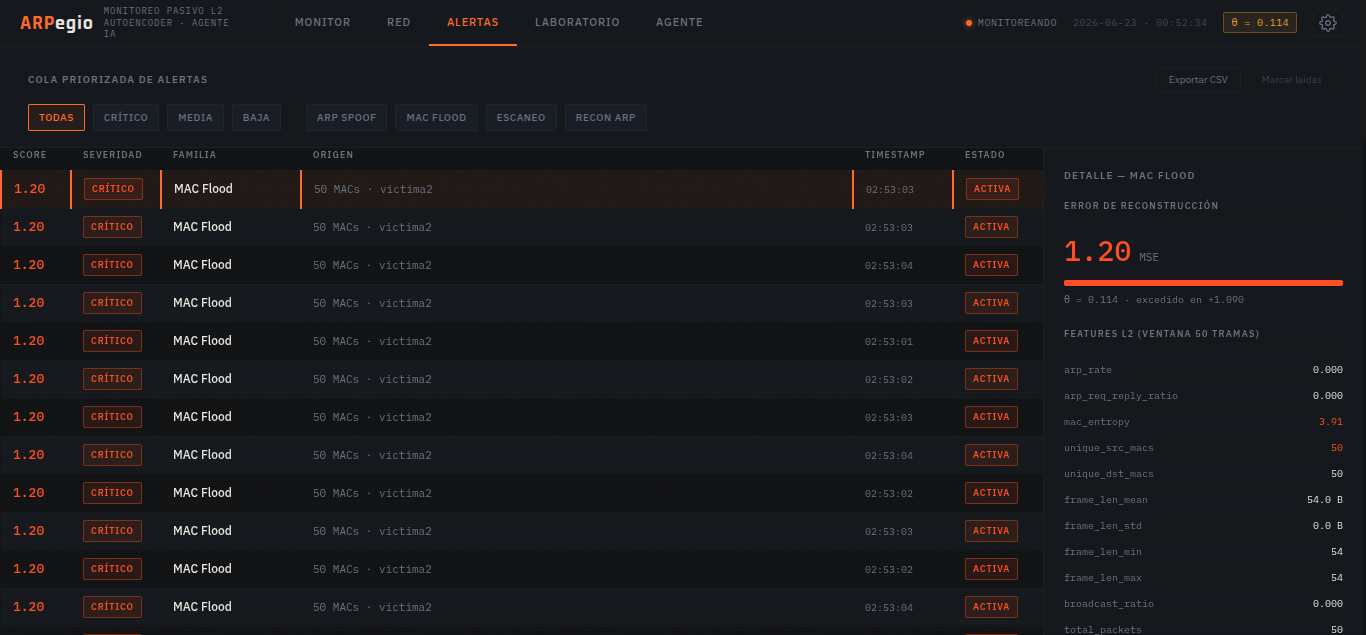
\includegraphics[width=\linewidth]{figs/alertas.png}
\caption{Vista Alertas: cola priorizada, filtros operativos y detalle
de la ventana seleccionada.}
\label{fig:platform_alerts}
\end{figure}

\subsection{Laboratorio interactivo con inferencia en el cliente}
La vista \textbf{Laboratorio} reproduce escenarios reales de la
captura---\arpspoof, \macflood, \portscan, \arprecon{} y tráfico
\trafonormal---mediante inferencia del \textit{autoencoder} en el
navegador. El modelo exportado se ejecuta íntegramente en el cliente,
sin enviar tráfico ni vectores de \textit{features} a un servidor
remoto. Un control de percentiles recalcula $\theta$ al vuelo y compara
el MSE reconstruido frente al umbral elegido; el escenario de
\portscan{} permanece documentado como caso de falso negativo honesto
cuando el punto de observación no captura la señal dominante. La
Fig.~\ref{fig:platform_lab} resume esta capacidad de validación
interactiva.

\begin{figure}[htbp]
\centering
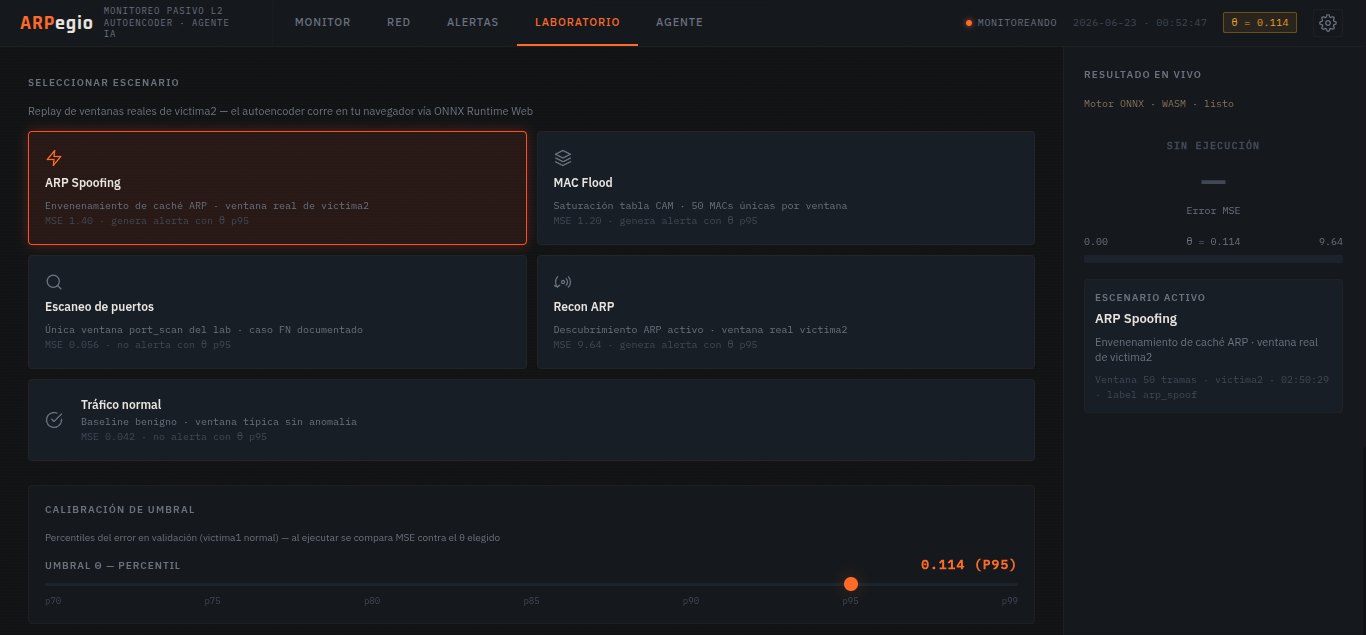
\includegraphics[width=\linewidth]{figs/laboratorio.png}
\caption{Vista Laboratorio: \textit{replay} de escenarios reales con
inferencia en el navegador y calibración interactiva de $\theta$.}
\label{fig:platform_lab}
\end{figure}

\subsection{Agente de asistencia y configuración}
La vista \textbf{Agente} integra un copiloto conversacional con modelo
de lenguaje (\textit{bring your own key}): la credencial permanece en
el navegador del operador y no transita por el servidor de la demo. Se
distinguen dos modos de operación:
\textbf{preventivo}---calibración de $\theta$, análisis de falsos
positivos y checklist pre-incidente---y
\textbf{reactivo}---planes de contención L2 y comandos sugeridos para el
laboratorio tras una alerta. El agente emite informes estructurados con
veredicto, nivel de confianza, recomendación de umbral, escenario de
laboratorio sugerido, acciones priorizadas y comandos de verificación.
Además, puede simular distintos percentiles de $\theta$, consultar
alertas individuales, listar la cola priorizada y recuperar el perfil
de escenarios del laboratorio a partir del estado vigente del sistema. Un
diálogo de seguimiento permite refinar las respuestas; la interfaz
presenta notación matemática y comandos de forma legible para el
operador. Accesos contextuales desde \textbf{Monitor}, \textbf{Alertas}
y \textbf{Laboratorio} abren el agente con la situación ya cargada. La
ejecución remota de mitigaciones en GNS3 no está automatizada: el agente
asiste al operador, pero la contención sigue siendo manual. La
Fig.~\ref{fig:platform_agent} muestra el flujo de informe en modo
reactivo.

La vista \textbf{Ajustes} centraliza la credencial del agente,
parámetros de modelo de solo lectura (arquitectura $11 \to 8 \to 4 \to 8 \to 11$,
AUC, $\theta$ activo) y acceso a la documentación del proyecto y a las
capturas del laboratorio. La Fig.~\ref{fig:platform_settings} corresponde
a este panel.

\begin{figure}[htbp]
\centering
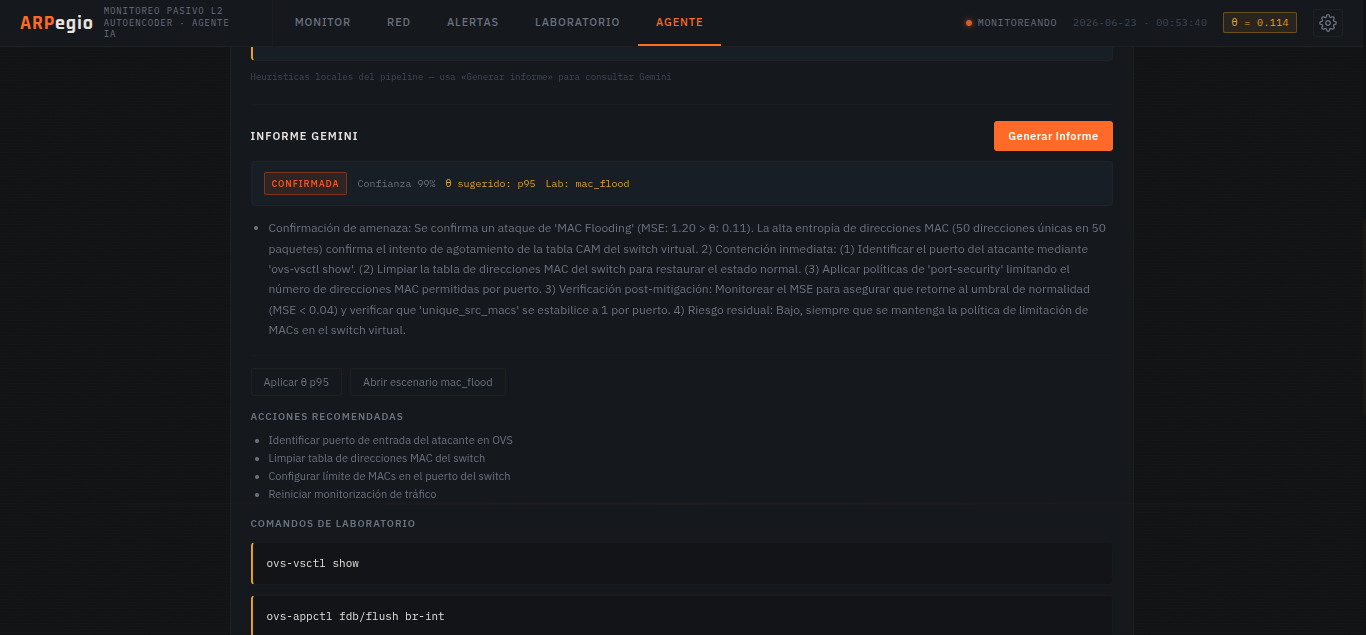
\includegraphics[width=\linewidth]{figs/agente.png}
\caption{Vista Agente: modos preventivo y reactivo, informe estructurado
y diálogo de seguimiento con consulta al estado del sistema.}
\label{fig:platform_agent}
\end{figure}

\begin{figure}[htbp]
\centering
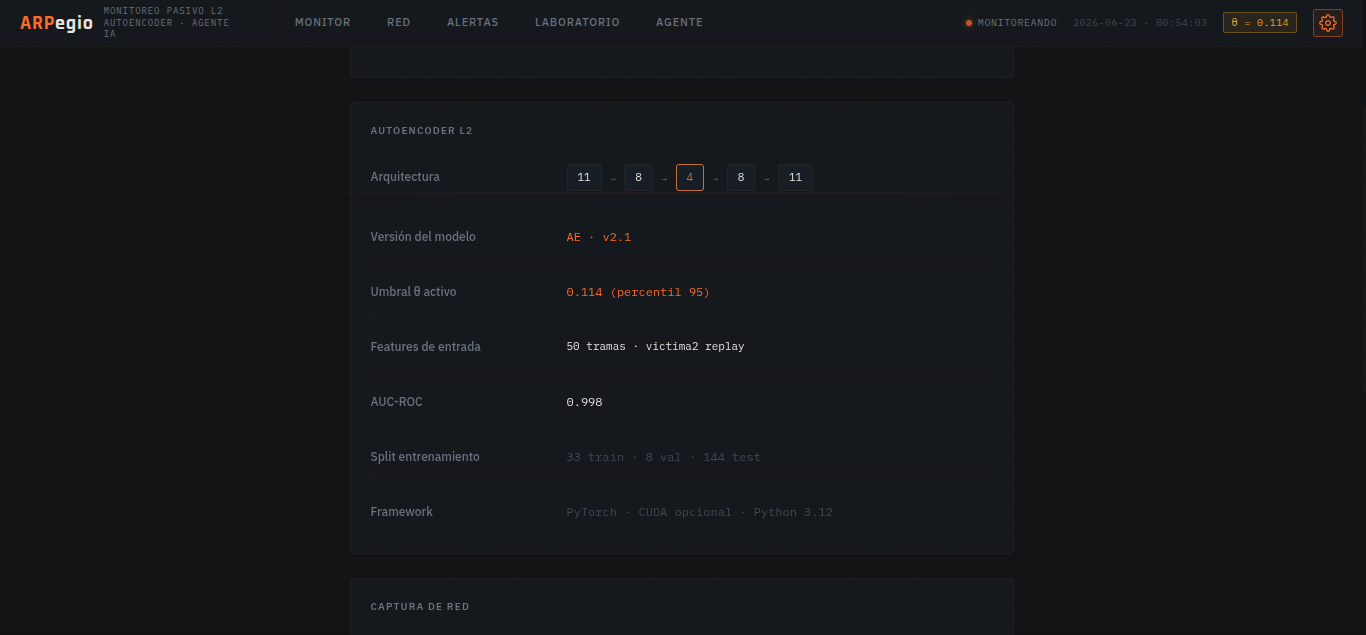
\includegraphics[width=\linewidth]{figs/ajustes.png}
\caption{Vista Ajustes: configuración del agente, metadatos del
\textit{autoencoder} y acceso a documentación del proyecto.}
\label{fig:platform_settings}
\end{figure}

% ---------------------------------------------------------------
%  VI. RESULTADOS Y DISCUSIÓN
% ---------------------------------------------------------------
\section{Resultados y Discusión}

\subsection{Entrenamiento del \textit{autoencoder}}
El modelo convergió en 100 épocas con pérdida MSE final de
$3{,}9\times10^{-2}$ sobre 33 ventanas de \trafonormal{} de la
\victimauno. La Fig.~\ref{fig:loss} muestra la curva de
entrenamiento monótonamente decreciente, sin sobreajuste aparente dado
el reducido tamaño del conjunto de entrenamiento no supervisado.

\begin{figure}[htbp]
\centering
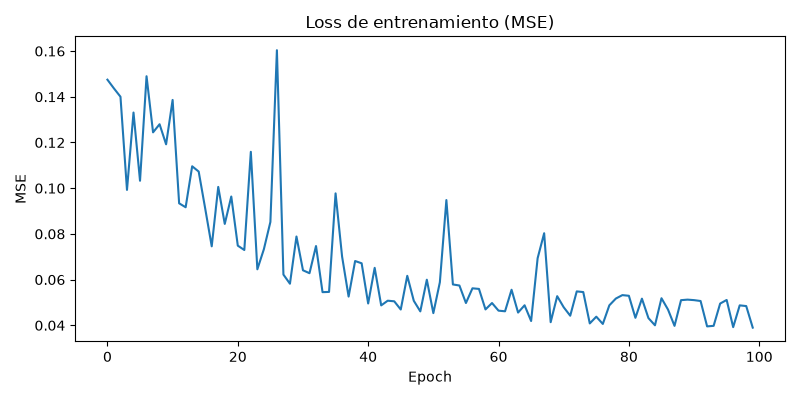
\includegraphics[width=\linewidth]{figs/training_loss.png}
\caption{Curva de pérdida MSE durante el entrenamiento (100 épocas).}
\label{fig:loss}
\end{figure}

\subsection{Calibración del umbral y separabilidad}
El umbral $\theta = 0{,}114$ se obtuvo como percentil~95 del error MSE
sobre ocho ventanas normales de validación (perspectiva de la
\victimauno, no vistas en entrenamiento). La Fig.~\ref{fig:errors} contrasta la
distribución de errores normales frente a ventanas de ataque en la
\victimados: las familias ARP y \macflood{} quedan
claramente separadas del tráfico legítimo.

\begin{figure}[htbp]
\centering
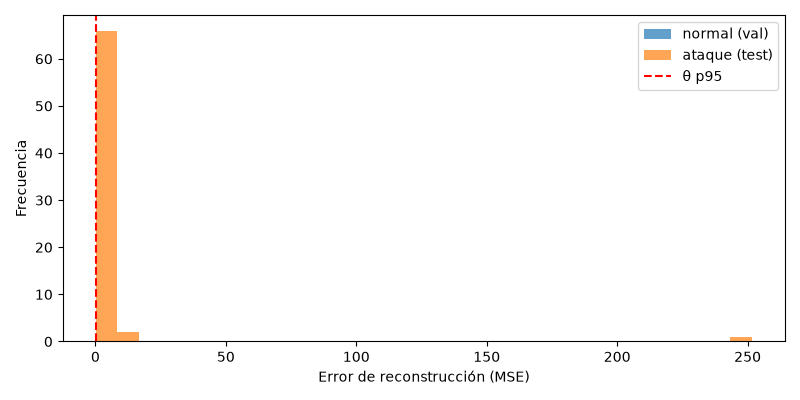
\includegraphics[width=\linewidth]{figs/reconstruction_errors.png}
\caption{Distribución del error de reconstrucción: validación normal vs.
ataques en la segunda víctima; línea vertical en $\theta$.}
\label{fig:errors}
\end{figure}

\subsection{Detección binaria y AUC}
Sobre 144 ventanas de prueba (perspectiva de la \victimados), la clasificación
binaria normal/ataque alcanzó precisión, \textit{recall}
y F1 de 0.97 en ambas clases (exactitud global 97\%). El AUC-ROC fue
0{,}9986, indicando excelente capacidad discriminativa del error de
reconstrucción como estadístico de anomalía.

\subsection{Detección por familia de ataque}
La Tabla~\ref{tab:deteccion_clase} resume la tasa de detección por
etiqueta de evaluación. Tres de las cuatro familias de ataque L2
alcanzaron detección perfecta en la \victimados. No obstante, dado
que \arpspoof{} cuenta con únicamente tres ventanas en el
conjunto de prueba, este resultado debe interpretarse con cautela
estadística. La ausencia de detección en \portscan{} (0/1)
refleja la baja visibilidad de este ataque desde la perspectiva de la
\victimados, donde solo una ventana fue etiquetada para esta
clase; no constituye un fallo del modelo sino una limitación del punto
de observación (36 ventanas en el \textit{dataset} completo frente a
795 de \macflood).

\begin{table}[htbp]
\caption{Detección por familia de ataque (segunda víctima, $\theta=0{,}114$)}
\label{tab:deteccion_clase}
\centering
\renewcommand{\arraystretch}{1.15}
\begin{tabular}{lrrr}
\hline
\textbf{Clase de tráfico} & \textbf{Detectadas} & \textbf{Total} & \textbf{Tasa (\%)} \\
\hline
MAC flooding  & 62 & 62 & 100.0 \\
ARP spoofing  &  3 &  3 & 100.0 \\
Reconocimiento ARP  &  3 &  3 & 100.0 \\
Escaneo de puertos  &  0 &  1 &   0.0 \\
Tráfico normal (FP) &  3 & 75 &   4.0 \\
\hline
\end{tabular}
\end{table}

Los tres falsos positivos sobre 75 ventanas normales (4\%) se sitúan
dentro del margen esperado para un percentil~95 de calibración sobre un
subconjunto pequeño de validación.

\subsection{Motor de priorización}
Tras aplicar el motor de la ecuación~\eqref{eq:priority} sobre las 71
alertas generadas en la \victimados---62 de \macflood, tres de
\arpspoof, tres de \arprecon{} y tres falsos positivos
sobre \trafonormal---las ventanas de \macflood{}
persistente obtuvieron puntaje máximo ($P=1{,}0$) por
combinar severidad, frecuencia deslizante e impacto operacional elevado.
Las alertas ARP aparecieron con menor frecuencia acumulada pero mantuvieron
prioridad alta gracias a $s \approx 1$ e impacto $i \geq 0{,}6$. El
ordenamiento descendente por $P$ permite al operador atender primero
ráfagas sostenidas de inundación MAC antes que eventos aislados de baja
severidad, mitigando el \textit{alert fatigue}~\cite{tariq2025}.

\subsection{Integración de resultados en la plataforma}
Los indicadores cuantitativos anteriores no permanecen confinados a
informes estáticos: la plataforma \textit{ARPegio} los traduce a una
superficie operativa coherente con el flujo de trabajo de un SOC. La
vista \textbf{Monitor} reproduce de forma inmediata el AUC-ROC de
0{,}998, el umbral $\theta$ calibrado, el volumen de alertas y la tasa
de falsos positivos del 4\%, junto con un histograma que visualiza la
misma separabilidad entre tráfico normal y ataques discutida en la
Fig.~\ref{fig:errors}. Un control interactivo de percentiles permite al
analista explorar, sin reentrenar el modelo, cómo varían los conteos
TN/FP/FN/TP al desplazar $\theta$---capacidad especialmente relevante
para negociar el compromiso entre sensibilidad y ruido operativo en
entornos con escasa muestra de validación.

La vista \textbf{Alertas} materializa el ordenamiento del motor de
priorización: las 71 ventanas anómalas de la \victimados{} aparecen
clasificadas por puntaje $P$, con filtros por severidad y familia de
ataque. Las tres alertas de mayor prioridad se destacan también en
\textbf{Monitor} como acceso directo al \textit{triage}, replicando la
lógica con la que un operador abordaría primero las ráfagas de
\macflood{} ($P=1{,}0$) frente a eventos ARP de menor persistencia.
La vista \textbf{Red} sitúa cada ventana en la topología GNS3 y en la
línea temporal de la sesión, ofreciendo contexto espacial y cronológico
que las métricas agregadas no capturan por sí solas. En conjunto, estas
vistas validan que el \textit{pipeline} experimental es interpretable
más allá de tablas y curvas de entrenamiento (Figs.~\ref{fig:platform_monitor}
y~\ref{fig:platform_alerts}).

\subsection{Validación interactiva y asistencia al operador}
La vista \textbf{Laboratorio} constituye el segundo eje de validación de
la plataforma: en lugar de consumir pasivamente los resultados del
\textit{replay} offline, el analista ejecuta la inferencia del
\textit{autoencoder} sobre escenarios reales de la captura y compara el
error de reconstrucción frente a distintos percentiles de $\theta$. Este
mecanismo reproduce en el cliente la decisión binaria normal/anomalía y
hace tangible el caso de \portscan{} no detectado desde la
\victimados: la interfaz documenta el falso negativo como limitación
del punto de observación, no como omisión del tablero. La
Fig.~\ref{fig:platform_lab} ilustra este enfoque de validación
transparente.

El módulo \textbf{Agente} cierra el ciclo con asistencia cognitiva en
dos modos complementarios. En régimen \textbf{preventivo}, orienta la
calibración de $\theta$, el análisis de falsos positivos y la
planificación pre-incidente; en régimen \textbf{reactivo}, propone
secuencias de contención L2 y comandos de verificación tras una alerta.
Los informes estructurados sintetizan veredicto, confianza, umbral
sugerido y acciones priorizadas, mientras el diálogo de seguimiento
permite refinar hipótesis---por ejemplo, contrastar el efecto de un
percentil más conservador sobre los falsos positivos observados. Los
accesos contextuales desde \textbf{Monitor}, \textbf{Alertas} y
\textbf{Laboratorio} reducen la fricción entre detección, priorización
e interpretación. La Fig.~\ref{fig:platform_agent} muestra este flujo en
modo reactivo. La vista \textbf{Ajustes} concentra la configuración del
agente y los metadatos del modelo para auditoría reproducible
(Fig.~\ref{fig:platform_settings}).

Desde una perspectiva de usabilidad, la plataforma demuestra que los
resultados del experimento GNS3 pueden transferirse a un entorno
accesible vía Web sin sacrificar la trazabilidad del modelo: cada
indicador mostrado deriva del mismo umbral, la misma arquitectura
$11 \to 8 \to 4 \to 8 \to 11$ y la misma cola priorizada evaluada en
esta sección. El despliegue público facilita la revisión por pares del
comportamiento operativo del sistema, más allá de la lectura de métricas
aisladas.

\subsection{Limitaciones}
El tamaño reducido de clases minoritarias (\arpspoof,
\arprecon{} y \portscan) limita la generalización
estadística. La validación cruzada por víctima (\victimauno{} $\to$
\victimados) demuestra transferencia entre perspectivas de captura,
pero no sustituye un despliegue en producción con mayor diversidad
topológica.

En el plano de la plataforma, la inferencia en el navegador y la carga
estática de resultados del \textit{pipeline} la orientan hacia demostración,
capacitación y \textit{triage} sobre capturas ya procesadas, no hacia
monitoreo en tiempo real de alto caudal. El agente de asistencia opera
con credencial aportada por el operador y no ejecuta mitigaciones de
forma autónoma en el laboratorio: su valor reside en la interpretación y
la propuesta de acciones, no en la orquestación remota de contención. La
integración con flujos SOC empresariales (SIEM, \textit{ticketing},
autenticación institucional) permanece como trabajo pendiente.

% ---------------------------------------------------------------
%  VII. CONCLUSIONES
% ---------------------------------------------------------------
\section{Conclusiones}

Este trabajo consolidó un \textit{pipeline} reproducible de detección de
anomalías L2 en redes LAN IEEE~802.3: captura pasiva en laboratorio GNS3,
extracción de 11 \textit{features} Ethernet nativas, entrenamiento no
supervisado con \textit{autoencoder} y calibración estadística del umbral
sin muestras de ataque. Sobre tráfico de la \victimados{} no visto en
entrenamiento, el sistema alcanzó 97\% de exactitud binaria y AUC-ROC de
0.998, detectando por completo \macflood, \arpspoof{} y
\arprecon---si bien \arpspoof{} y \arprecon{}
cuentan con muestras de prueba reducidas ($n=3$ cada una)---, con una
tasa de falsos positivos del 4\% sobre tráfico normal.

La integración de un motor de priorización por severidad, frecuencia e
impacto ordenó 71 alertas sin intervención humana ni etiquetas en
inferencia, demostrando que el \textit{alert fatigue} puede mitigarse
incluso con un subconjunto acotado de validación. Más allá del núcleo
analítico, la plataforma \textit{ARPegio} materializa estos hallazgos en
una experiencia operativa de extremo a extremo: el analista supervisa
métricas y separabilidad del modelo, explora el compromiso del umbral de
forma interactiva, recorre la cola priorizada con contexto topológico,
reproduce escenarios de laboratorio con inferencia en el cliente y recibe
asistencia del agente en modos preventivo y reactivo. Esta capa de
presentación no sustituye la evaluación cuantitativa de las
subsecciones anteriores, sino que la hace accionable para un perfil de
usuario no especializado en aprendizaje automático.

Los resultados confirman que el monitoreo pasivo anclado en tramas
IEEE~802.3 es viable para alertar tempranamente sobre ataques de
suplantación y saturación en LAN institucionales simuladas. La
combinación de detección no supervisada, priorización heurística e
interfaz de operación constituye una respuesta coherente a la brecha
identificada en la literatura: sistemas L2 sin agentes en los nodos,
sin dependencia de etiquetas en entrenamiento y con un camino claro
desde la anomalía detectada hasta la decisión del analista.

Como líneas futuras se identifican: ampliar capturas para \portscan{} y
clases minoritarias; incorporar alimentación en tiempo real o
\textit{streaming} de ventanas L2 a la plataforma; automatizar la
ejecución supervisada de mitigaciones sugeridas por el agente en el
laboratorio GNS3; integrar autenticación institucional y exportación hacia
SIEM; y validar el motor de priorización con roles heterogéneos
(servidor/cliente/IoT) en topologías más amplias. En conjunto, el
trabajo aporta evidencia experimental y un prototipo operativo que
acercan la detección de anomalías en capa de enlace a un escenario
institucional verificable y comunicable.

% ---------------------------------------------------------------
%  REFERENCES
% ---------------------------------------------------------------
\begin{thebibliography}{00}

% --- Referencias de la Introducción ---

\bibitem{tufan2021}
E.~Tufan, C.~Tezcan, and C.~Acartürk,
``Anomaly-Based Intrusion Detection by Machine Learning: A Case Study
on Probing Attacks to an Institutional Network,''
\textit{IEEE Access},
vol.~9, pp.~50078--50092, 2021.

\bibitem{gamage2020}
S.~Gamage and J.~Samarabandu,
``Deep learning methods in network intrusion detection: A survey and an
objective comparison,''
\textit{Journal of Network and Computer Applications},
vol.~169, p.~102767, 2020.

\bibitem{sarhan2022}
M.~Sarhan, S.~Layeghy, and M.~Portmann,
``Towards a Standard Feature Set for Network Intrusion Detection System
Datasets,''
\textit{Mobile Networks and Applications},
vol.~27, pp.~357--370, 2022.

\bibitem{he2023}
K.~He, D.~D. Kim, and M.~R. Asghar,
``Adversarial Machine Learning for Network Intrusion Detection Systems:
A Comprehensive Survey,''
\textit{IEEE Communications Surveys \& Tutorials},
vol.~25, no.~1, pp.~538--566, First Quarter 2023.

\bibitem{morsy2022}
S.~M. Morsy and D.~Nashat,
``D-ARP: An Efficient Scheme to Detect and Prevent ARP Spoofing,''
\textit{IEEE Access},
vol.~10, pp.~49142--49153, 2022.

\bibitem{sakhawat2019}
D.~Sakhawat, A.~N. Khan, M.~Aslam, and A.~T. Chronopoulos,
``Agent-based ARP cache poisoning detection in switched LAN
environments,''
\textit{IET Networks},
vol.~8, no.~1, pp.~67--73, 2019.

\bibitem{tariq2025}
S.~Tariq, M.~B. Chhetri, S.~Nepal, and C.~Paris,
``Alert Fatigue in Security Operations Centres: Research Challenges
and Opportunities,''
\textit{ACM Computing Surveys},
vol.~57, no.~9, 2025.

\bibitem{injadat2021}
M.~Injadat, A.~Moubayed, A.~B. Nassif, and A.~Shami,
``Multi-Stage Optimized Machine Learning Framework for Network
Intrusion Detection,''
\textit{IEEE Transactions on Network and Service Management},
vol.~18, no.~2, pp.~1803--1816, Jun.~2021.

\bibitem{yang2022}
Z.~Yang, X.~Liu, T.~Li, D.~Wu, J.~Wang, Y.~Zhao, and H.~Han,
``A systematic literature review of methods and datasets for
anomaly-based network intrusion detection,''
\textit{Computers \& Security},
vol.~116, p.~102675, 2022.


% --- Referencias nuevas de Trabajos Relacionados ---
 
\bibitem{griffinyang2022}
L.~Griffin, Z.~Yang, Y.~Song, S.~Gao, A.~Hu, and B.~Xiao,
``Griffin: Real-Time Network Intrusion Detection System via
Ensemble of Autoencoder in SDN,''
\textit{IEEE Transactions on Network and Service Management},
vol.~19, no.~3, pp.~2269--2282, Sep.~2022.
 
\bibitem{antunes2022}
M.~Antunes, L.~Oliveira, A.~Seguro, J.~Veríssimo, R.~Salgado,
and T.~Murteira,
``Benchmarking Deep Learning Methods for Behaviour-Based Network
Intrusion Detection,''
\textit{Informatics},
vol.~9, no.~1, p.~29, 2022.
 
\bibitem{sun2021ojcoms}
Y.~Sun, H.~Esaki, and H.~Ochiai,
``Adaptive Intrusion Detection in the Networking of Large-Scale LANs
With Segmented Federated Learning,''
\textit{IEEE Open Journal of the Communications Society},
vol.~2, pp.~102--112, 2021.
 
\bibitem{prasad2022}
A.~Prasad and S.~Chandra,
``Defending ARP Spoofing-based MitM Attack using Machine Learning
and Device Profiling,''
in \textit{2022 International Conference on Computing, Communication,
and Intelligent Systems (ICCCIS)}, 2022, pp.~978--983.
 
\bibitem{sun2022ccnc}
Y.~Sun, H.~Ochiai, and H.~Esaki,
``Suspicious ARP Activity Detection and Clustering Based on Autoencoder
Neural Networks,''
in \textit{IEEE Consumer Communications \& Networking Conference
(CCNC)}, 2022.
 
\bibitem{aminanto2020}
M.~E. Aminanto, T.~Ban, R.~Isawa, T.~Takahashi, and D.~Inoue,
``Threat Alert Prioritization Using Isolation Forest and Stacked Auto
Encoder With Day-Forward-Chaining Analysis,''
\textit{IEEE Access},
vol.~8, pp.~217977--217986, 2020.
 
\bibitem{jalalvand2024}
F.~Jalalvand, M.~B. Chhetri, S.~Nepal, and C.~Paris,
``Alert Prioritisation in Security Operations Centres: A Systematic
Survey on Criteria and Methods,''
\textit{ACM Computing Surveys},
vol.~57, no.~2, pp.~1--36, 2024.
 
\bibitem{carrera2022}
F.~Carrera et al.,
``Combining Unsupervised Approaches for Near Real-Time Network Traffic
Anomaly Detection,''
\textit{Applied Sciences},
vol.~12, no.~3, p.~1759, 2022.

% --- Nuevas referencias de Metodología ---

\bibitem{li2020}
X.~Li, W.~Chen, Q.~Zhang, and L.~Wu,
``Building Auto-Encoder Intrusion Detection System Based on Random
Forest Feature Selection,''
\textit{Computers \& Security},
vol.~95, p.~101851, 2020.

\bibitem{song2021}
Y.~Song, C.~Hyun, and Y.~Cheong,
``Self-Supervised Anomaly Detection with Neural Transformation
Learning for Log-Based Intrusion Detection,''
\textit{IEEE Access},
vol.~9, pp.~53127--53143, 2021.

\bibitem{maleki2021}
N.~Maleki, M.~Zeinali, and S.~T.~Hasson,
``A Kind of Threshold-Based Anomaly Detection in Autoencoder,''
in \textit{2021 5th International Conference on Pattern Recognition
and Image Analysis (IPRIA)}, 2021, pp.~1--6.

\bibitem{zavrak2020}
S.~Zavrak and M.~{\.I}skefiyeli,
``Anomaly-Based Intrusion Detection From Network Flow Features
Using Variational Autoencoder,''
\textit{IEEE Access},
vol.~8, pp.~108346--108358, 2020.

\bibitem{zhang2023}
H.~Zhang, X.~Li, T.~Liu, and J.~Gu,
``Threshold Optimization in Autoencoder-Based Anomaly Detection
for Network Traffic,''
\textit{IEEE Transactions on Network and Service Management},
vol.~20, no.~2, pp.~1753--1765, Jun.~2023.

\end{thebibliography}

\end{document}